\begin{titlepage}
\begin{center}

% Upper part of the page. The '~' is needed because only works if a paragraph has started.
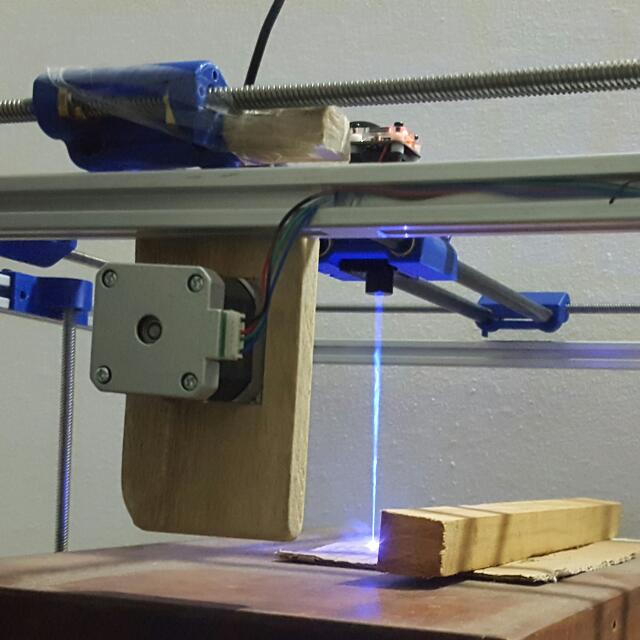
\includegraphics[width=0.35\textwidth]{./logo}~\\[1cm]

\textsc{\LARGE IFNTI - Sokodé}\\[1.5cm]

\textsc{\Large }\\[0.5cm]

% Title
\HRule \\[0.4cm]

{\huge \bfseries Imprimante 3D - Laser\\
Conception d'une imprimante 3D et d'une Graveuse Laser \\[0.4cm] }

\HRule \\[1.5cm]

% Author and supervisor
\begin{minipage}{0.4\textwidth}
\begin{flushleft} \large
\emph{Auteurs:}\\
\textsc{AYEVA Yaasiin}\\
\textsc{ISSA-TOURÉ Aziz}\\
\textsc{TCHASSONA TRAORÉ Walid}\\
\textsc{TÉOURI Samrou}\\
\textsc{TÉOURI Touré-Ydaou}
\end{flushleft}
\end{minipage}
\begin{minipage}{0.4\textwidth}
\begin{flushright} \large
\emph{Client:} \\
\textsc{IFNTI}\\
\emph{Référent:} \\
\textsc{Jean-Christophe CARRE}
\end{flushright}
\end{minipage}

\vfill

% Bottom of the page
{\large \today}

\end{center}
\end{titlepage}